%% The following is a directive for TeXShop to indicate the main file
%%!TEX root = SPIE_2014_lukasc_v2b.tex
\graphicspath{{figs_chris/}}


%%%%%%%%%%%%%%%%%%%%%%%%%%%%%%%%%%%%%%%%%%%%%%%%%%%%%%%%%%%%%%%%%%%%%%
\section{Fabrication Variability and Yield Predication for Silicon Photonic MZI Switches}
\label{sec:variability}
The high refractive index contrast of SOI permits sharp waveguide bends and ultrasmall device sizes, making it promissing for the development of dense integration of photonic components. However, silicon photonic devices face serious reliability challenges. Fabrication errors on either the waveguide linewidth or thickness might affact the propagation constant of light inside the waveguide, and, thus, degrade the performance of devices. 

Yield simulation and prediction are critical for photonic devices. In semiconductor manufacturing community, corner analysis and simple Monte Carlo simulation are typically used to analyze fabrication variability, the former of which predicts the worst performance of devices; while the later of which assume a uniform process variation across a wafer. However, neither of them captures die-to-die, device-to-device, and intra-device correlated variations. Correlated yield analysis is driving more and more attention, and some statistical investigations regarding on-chip correlation \cite{lukas14:OFC, hochberg14:wafer} and uncertainty of devices have been reported. In this work, we propose, for the first time, a correlated and physical layout dependent methodology for the yield analysis of on-chip photonic integrated circuits. From physical layout to Monte Carlo simulation, our methodology will provides an insight into the significance of compact layout for photonic designs, and offers a useful tool for post-layout verification and power trimming estimation.

\begin{figure}[h]
    \centering
    \label{flow_chart}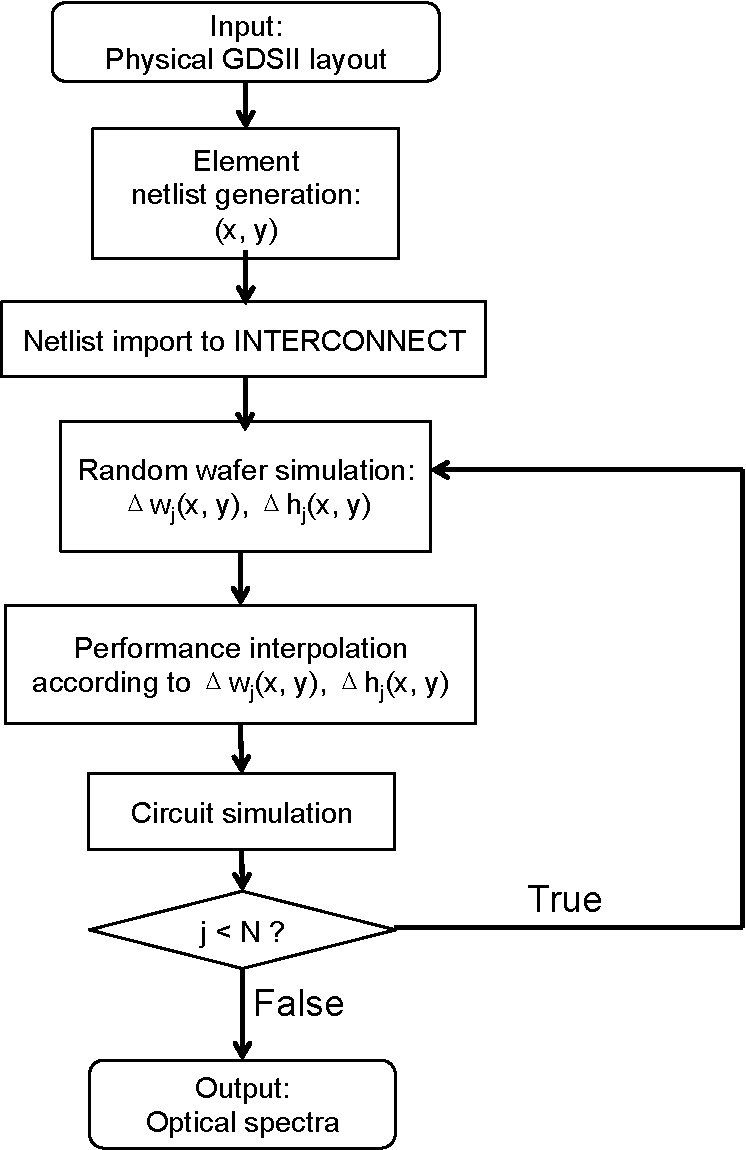
\includegraphics[width=13cm]{flow_chart.pdf}
    \vspace{-10pt}
    \caption{(a) Flow chart of the proposed methodology; (b) simulated waveguide linewidth deviations across a wafer; (c) simulated waveguide thickness deviations across a wafer.}
    \label{flow_chart}  
\end{figure}

Figure \ref{flow_chart}(a) shows the flow chart of our proposed methodology, and the procedures include: 
\begin{itemize}
\item First, silicon photonic circuits and/or devices under test are layouted using Klayout \cite{www_klayout}, an open-source graphic tool. 
\item
The netlist of the layout, which provides information about the primitive elements and the connections between the elements, are generated from Klayout and imported into Lumerical INTERCONNECT \cite{lumericalINTERCONNECT} for circuit simulation. 
\item
The third step is wafer simulation. In INTERCONNECT, silicon linewidth deviations, $\Delta w(x,y)$, and thickness deviations, $\Delta h(x,y)$, are simulated across the whole wafer, as demoed in Figs. \ref{flow_chart}(b) and \ref{flow_chart}(c), respectively. The simulated deviations are characterized by a sigma RMS amplitude and a correlation length, and both of them are based on experimental results \cite{NRCreview, hochberg14:wafer}. In each run of the Monte Carlo simulation, different deviation maps will be generated. 
\item
According to the spatial dependent linewidth and thickness deviations, the optical S-parameters of primitive elements and the optical propagation constants of connecting waveguides are interpolated in INTERCONNECT. 
\item
Finally, the interpolated circuit will be simulated. 
\end{itemize}

\begin{figure}[t]
    \centering
    \label{error}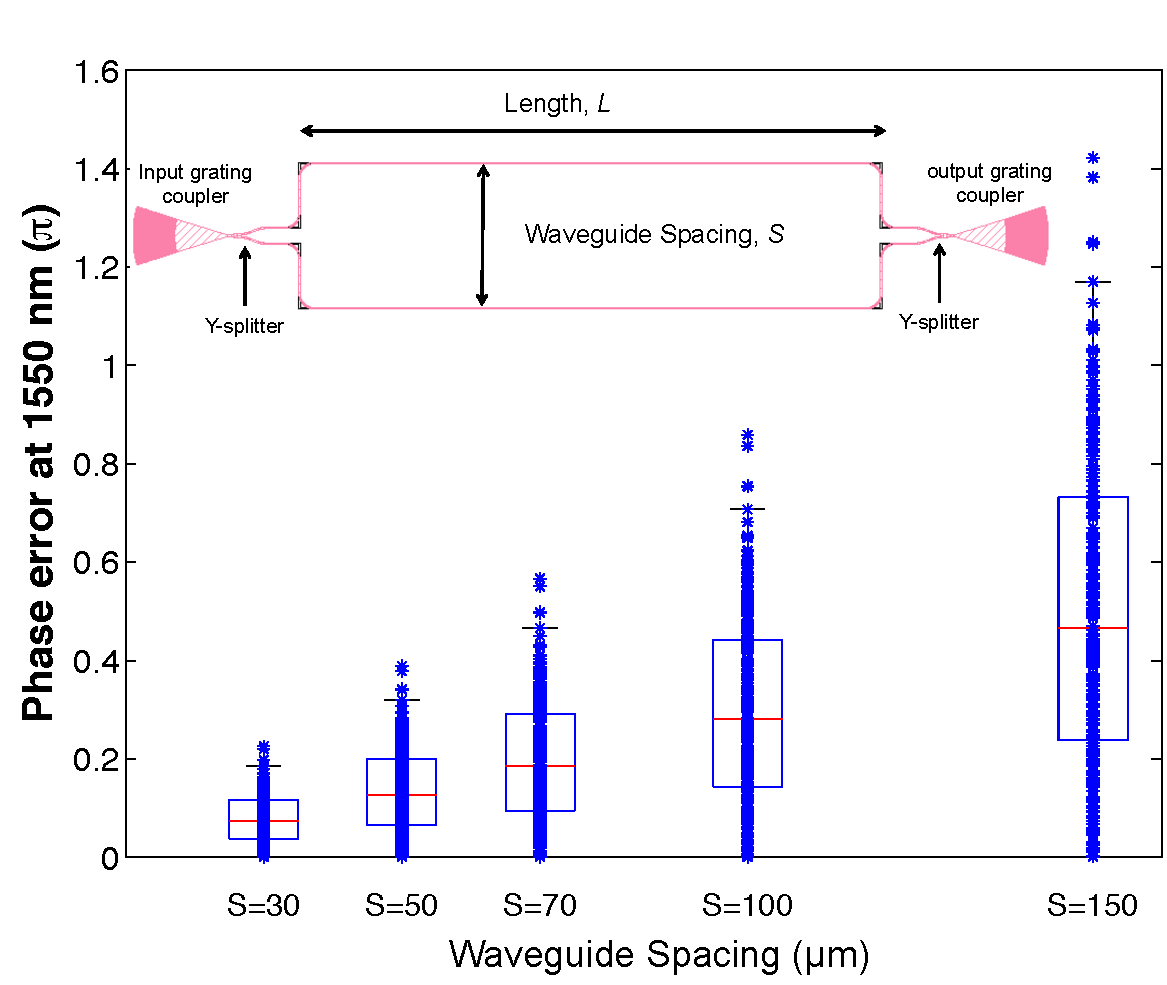
\includegraphics[width=8cm]{error.pdf}
    \caption{Scatter plot of phase error of a balanced MZI versus waveguide spacing.} 
    \label{error}
\end{figure}


The scatter plot in Fig. \ref{error} shows the simulated phase error of a balanced MZI versus the waveguide spacing between two phase arms, in a 248 nm CMOS compatible process. In the Monte Carlo simulations, the horizontal length of the phase arms, $L$,  is 200 $\mu m$. The phase error is defined as the absolute optical phase difference between the two phase arms. Ideally, the phase error should be 0 when there is no fabrication variation. However, this figure clearly shows that the phase error of the MZI is approximately linearly proportional to the waveguide spacing, emphasizing the significance of very compact layout designs. Additionally, the simulated phase error can be used to estimate the trimming power of MZI based photonic switches. 
